\chapter{Bluetooth}

\section{Description}

Bluetooth sensors are devices that utilize Bluetooth technology to wirelessly transmit data over short distances. They are commonly used in various applications including health monitoring, fitness tracking, smart home automation, industrial monitoring, and asset tracking. \cite{bluetoothPortentaH7:2024}
\newline
\textbf{Key Features:} \newline
\begin{itemize}

\item \textbf{Integrated BLE Module:} The Portenta H7 includes a built-in Bluetooth module that supports BLE, allowing for low-power, short-range wireless communication. It enables the board to interface with smartphones, tablets, and other BLE devices. 

\item \textbf{High Performance:} Equipped with a dual-core ARM Cortex-M7 and Cortex-M4 processor, the Portenta H7 provides robust processing power to handle complex tasks, including Bluetooth communications and data processing. 

\item \textbf{Easy Integration:} The Portenta H7 is compatible with the Arduino ecosystem, allowing for easy programming and integration with other Arduino shields and modules, including those utilizing Bluetooth communication. \cite{bluetoothPortentaH7:2024}

\end{itemize}

\section{Specific Sensor}
The BLE functionality in the Portenta H7 is provided by an integrated module that adheres to the Bluetooth 5.0 standard. This module supports features such as enhanced range, increased speed, and improved data throughput compared to previous Bluetooth versions.
\newline
The onboard Bluetooth module of the Portenta H7 offers low energy Bluetooth functionality, in order to provide the board with the flexibility to be easily connected to devices which also support Bluetooth Low Energy, such as the Arduino Nano 33 IoT or most modern smartphones. Compared to classic Bluetooth, Low Energy Bluetooth is intended to provide considerably reduced power consumption and cost while maintaining a similar communication range. \cite{bluetoothPortentaH7:2024}

\section{Specification}

\begin{itemize}
	
	\item The BLE sensor on the Arduino Portenta H7 operates on the Bluetooth 5.0 standard.
	\item It is integrated into the board, eliminating the need for additional Bluetooth hardware.
	\item The BLE sensor supports various data transfer modes including Advertising, Scanning, and Connection.
	\item The module operates on a low power mode to ensure efficient energy usage.
	\item It provides a communication range of up to 100 meters in open space.
	\item The BLE sensor can be programmed using the Arduino IDE with appropriate libraries for BLE communication. \cite{bluetoothPortentaH7:2024}
	
\end{itemize}


\section{TESTS}
In the listing  ~\ref{LedControl}, the Bluetooth sensor is initialized and used to advertise a simple message. This basic setup demonstrates how to get started with BLE communication on the Portenta H7.

{
	\captionof{code}{Simple sketch to control the LED using bluetooth}\label{LedControl}
	\ArduinoExternal{}{../Code/Bluetooth/LedControl/LedControl.ino}
}


This is just a simple example. The necessary libraries such as \textcolor{red}{<ArduinoBLE.h>} should be included, and the BLE device name and services can be defined as per the application requirements. \cite{bluetoothPortentaH7:2024}


\textbf{Example}

\subsection{control the built-in LED using Bluetooth}
The onboard Bluetooth module of the Portenta H7 offers low energy Bluetooth functionality, in order to provide the board with the flexibility to be easily connected to devices which also support Bluetooth Low Energy, such as the Arduino Nano 33 IoT or most modern smartphones. Compared to classic Bluetooth, Low Energy Bluetooth is intended to provide considerably reduced power consumption and cost while maintaining a similar communication range. \cite{bluetoothPortentaH7:2024}

\subsubsection{Overview}
In this Example we will enable low energy Bluetooth  on the Portenta H7 to allow an external Bluetooth device to control the built-in LED either by turning it on or off. \cite{bluetoothPortentaH7:2024}

\subsubsection{Goals}
\begin{itemize}
	\item Enabling Bluetooth Low Energy connectivity on the Portenta H7.
	\item Connecting the Portenta to an external Bluetooth Low Energy Mobile Application (In this case nRF Connect by Nordic Semiconductor). \cite{bluetoothPortentaH7:2024}
\end{itemize}

\subsubsection {Required Hardware and Software}
\begin{enumerate}
	\item Portenta H7 or Portenta H7 Lite Connected 
	\item USB-C cable (either USB-A to USB-C or USB-C to USB-C)
	\item Arduino IDE 1.8.13+ or Arduino Pro IDE 0.0.4+
	\item Mobile device, phone or tablet
	\item nRFconnect or equivalent tool downloaded on your mobile device: nRF Connect for iOS or nRF Connect for android \cite{bluetoothPortentaH7:2024}
\end{enumerate}

\subsubsection{Instructions}
\begin{itemize}
	\item \textbf{Configuring the Development Environment:} To communicate with the Portenta H7 via Bluetooth, you need to upload a pre-built sketch that starts a Bluetooth  network and allows your mobile device, which will be used to control the LEDs, to connect to it refer figure ~\ref{Bluetooth-portentaH7}. The sketch uses the ArduinoBLE Library that enables the Bluetooth  Low Energy module and handles important functions, such as scanning, connecting and interacting with services provided by other devices. You will also be using a third party application (e.g. nRF Connect), running on your mobile device in order to connect your device to the board and help you control the built-in LED.  \cite{bluetoothPortentaH7:2024}
	
	\begin{figure}
		\begin{center}
			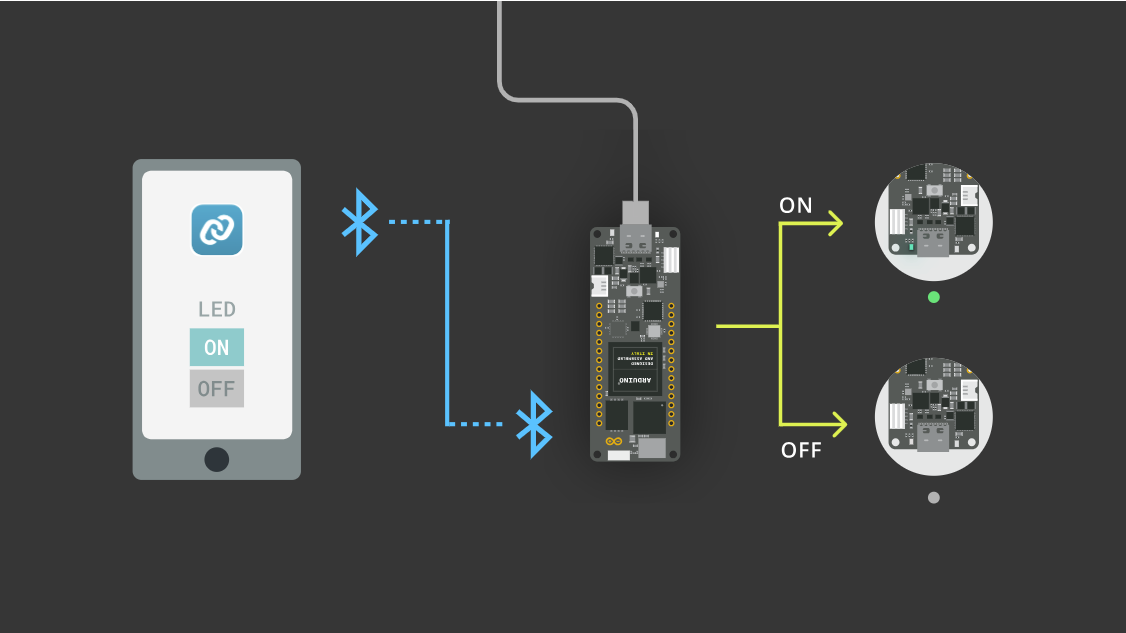
\includegraphics[width=0.7\linewidth]{Images/PortentaH7/Bluetooth-portentaH7.png}
			\caption{Bluetooth-portentaH7}
			\label{Bluetooth-portentaH7}\cite{bluetoothPortentaH7:2024}
		\end{center}
	\end{figure}
	
	\item \textbf{1. The Basic Setup:} Begin by plugging in your Portenta board to the computer using a USB-C cable and open the Arduino IDE. If this is your first time running Arduino sketch files on the board, we suggest you check out how to set up the Portenta H7 for Arduino before you proceed. ~\ref{PortentaH7-connection} \cite{bluetoothPortentaH7:2024}
	
	\begin{figure}
		\begin{center}
			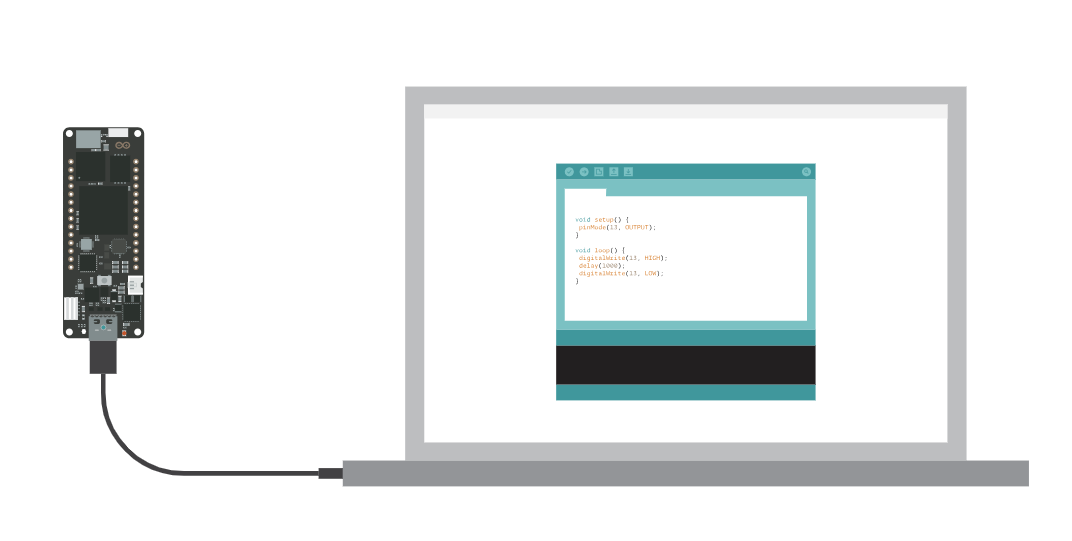
\includegraphics[width=0.7\linewidth]{Images/PortentaH7/PortentaH7-connection.png}
			\caption{PortentaH7-connection}
			\label{PortentaH7-connection} \cite{bluetoothPortentaH7:2024}
		\end{center}
	\end{figure}
	
	\item \textbf{2. Install the ArduinoBLE Library:} You will need to install the ArduinoBLE library in the Arduino IDE you are using. To install the library go to : \SHELL{ Tools > Manage Libraries...} type ArduinoBLE and click Install. Make sure you install ArduinoBLE version 1.1.3 or higher. ~\ref{Bluetooth-Library} \cite{bluetoothPortentaH7:2024}
	
	\begin{figure}
		\begin{center}
			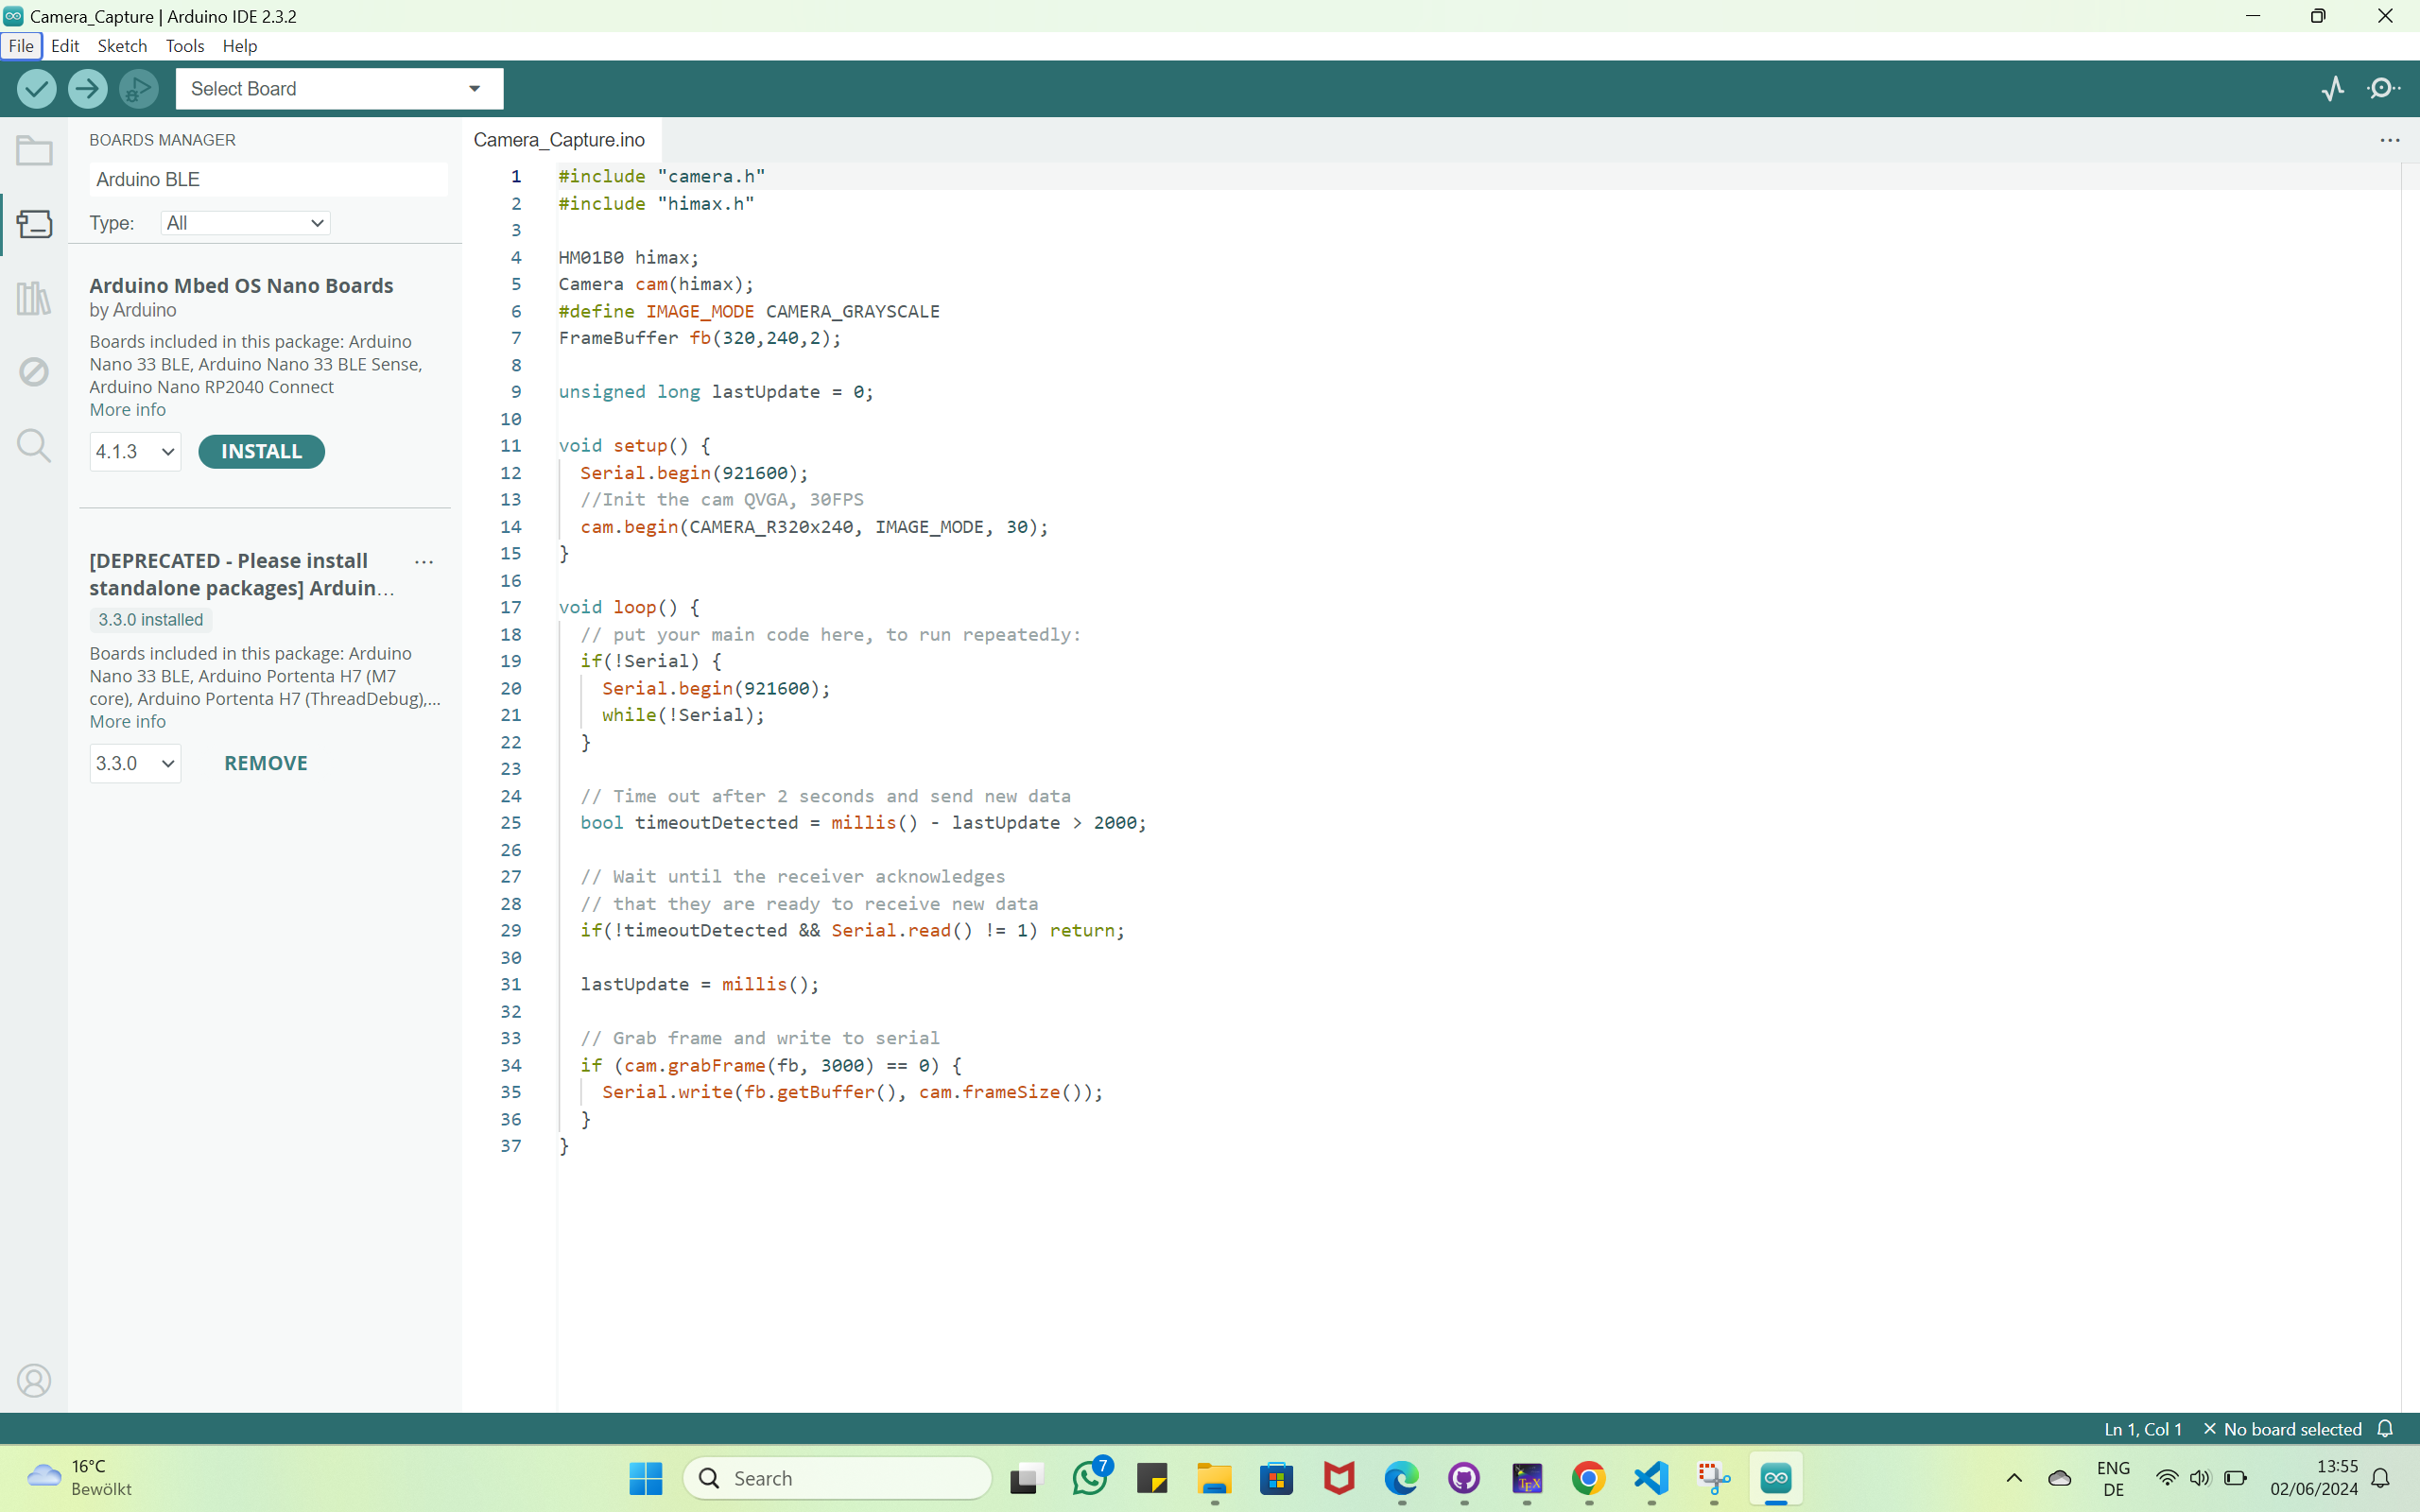
\includegraphics[width=0.7\linewidth]{Images/PortentaH7/Bluetooth-Library.png}
			\caption{Bluetooth-Library}
			\label{Bluetooth-Library}
		\end{center}
	\end{figure}
	
	\item \textbf{3. Create the Bluetooth Low Energy Sketch:} Let's program the Portenta with the following example sketch. If the Bluetooth  Low Energy module has been initialized correctly, you will see the blue LED lighting up for one second after uploading the sketch. If it fails, you will see the red LED lighting up instead. Copy and paste the following code into a new sketch in your IDE or download it from Arduino-Pro-Tutorials in the Arduino IDE and open it from: \SHELL{Examples > Arduino-Pro-Tutorials > BLE Connectivity on Portenta H7 > PortentaBLE } ~\ref{PortentaBLE} \cite{bluetoothPortentaH7:2024}
	
	{
		\captionof{code}{Simple sketch to control the LED using bluetooth}\label{PortentaBLE}
		\ArduinoExternal{}{../Code/Bluetooth/LedControl/PortentaBLE.ino}
	}
	
	
	In this example, you use a pre-defined Bluetooth number code pre-setup for controlling a device's LED. This code can also be referred to as GATT codes, which define how two Bluetooth  low energy devices transfer data. Once a connection is established with a device, its respective GATT code, which is a 16 bit identifier, is stored in a lookup table for future reference.
	
	These GATT codes are very long, but, in this example, it is always the same code: \cite{bluetoothPortentaH7:2024}
	
	\begin{lstlisting}[language=C++, frame=single, numbers=left, basicstyle=\ttfamily\small]
		BLEService ledService("19b10000-e8f2-537e-4f6c-d104768a1214"); // BLE LED Service
	\end{lstlisting}
	
	\item \textbf{4. Upload the Sketch:} Double press the reset button so the built-in LED is slowly pulsing green. Then, select your board in the menu: \SHELL{Tools > Board > Arduino Portenta H7 (M7 core)} ~\ref{Select-board-h7}
	\begin{figure}
		\begin{center}
			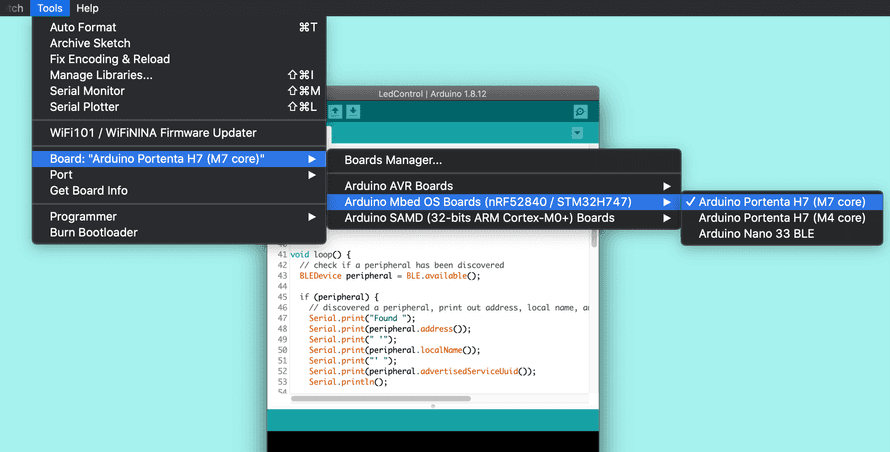
\includegraphics[width=0.7\linewidth]{Images/PortentaH7/select-board-h7.png}
			\caption{select-board-h7}
			\label{Select-board-h7} \cite{bluetoothPortentaH7:2024}
		\end{center}
	\end{figure}
	
	Choose the Port where your Portenta is connected to and Upload the sketch. Open the Serial Monitor once you have uploaded the code to the board to see debugging messages. If the Bluetooth  Low Energy setup was successful, you should see the message BLE LED Control ready. If something went wrong, you will see the message Starting Bluetooth Low Energy failed!. In that case update the Arduino BLE library (in the Library Manager) and the board (in the Board Manager) to the latest version and try again. ~\ref{select-port} \cite{bluetoothPortentaH7:2024}
	
	\begin{figure}
		\begin{center}
			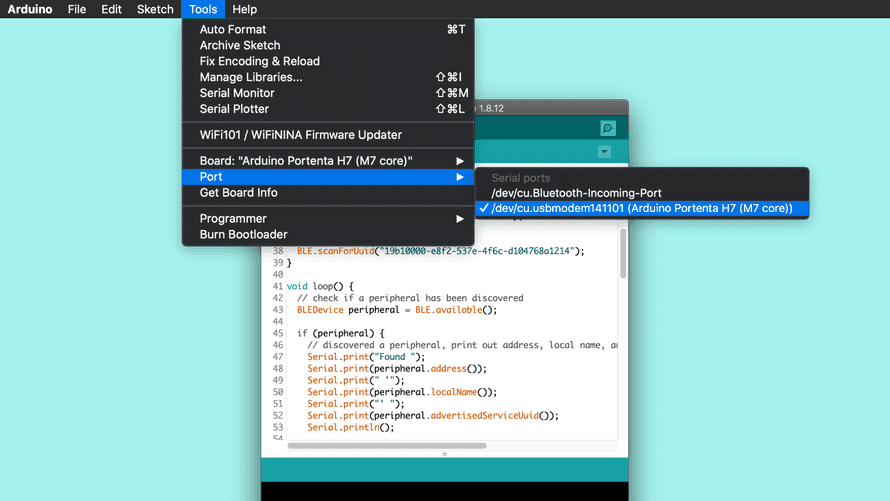
\includegraphics[width=0.7\linewidth]{Images/PortentaH7/select-port.png}
			\caption{Select the Port to which the Portenta is connected to}
			\label{select-port} \cite{bluetoothPortentaH7:2024}
		\end{center}
	\end{figure}
	
	\item \textbf{5.  Connect an External Device :} On your mobile device install nRF Connect or an equivalent app that allows for Bluetooth Low Energy connections. We will refer to nRF Connect for the rest of this tutorial. ~\ref{NRF-Connect} 
	
	\begin{figure}
		\begin{center}
			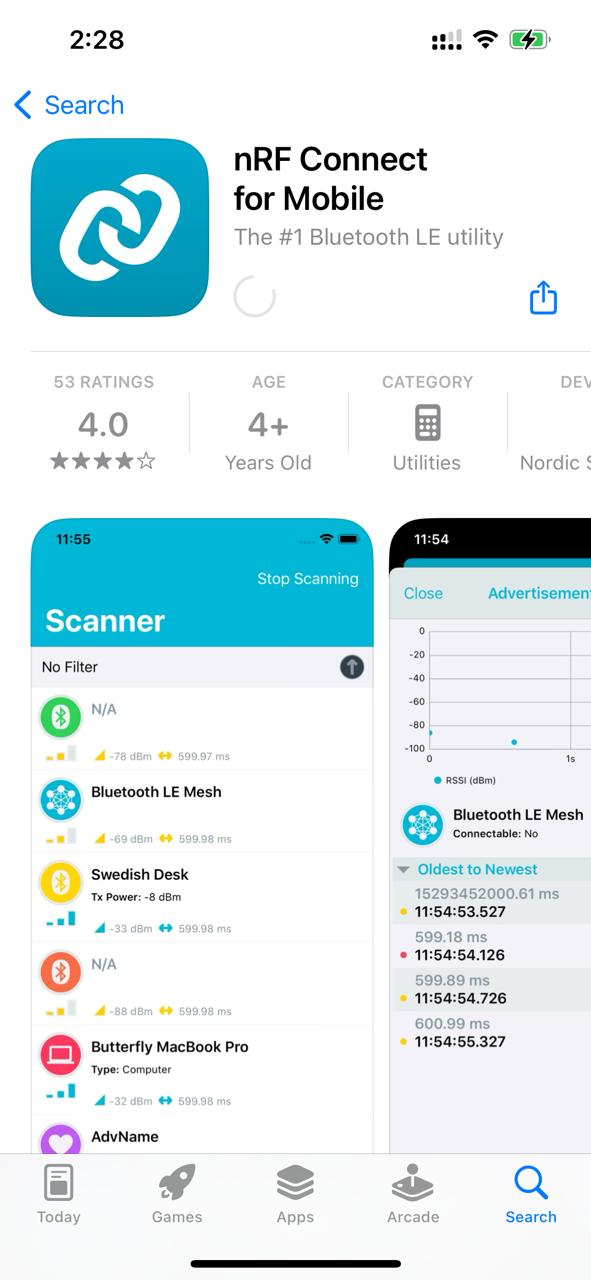
\includegraphics[width=0.7\linewidth]{Images/PortentaH7/NRF-Connect.jpg}
			\caption{NRF-Connect}
			\label{NRF-Connect}
		\end{center}
	\end{figure}
	
	Once you have downloaded the nRF application on your mobile device, look for your Portenta in the device list. You may filter the list by "Portenta" to easierly find your board in case you are using nRF Connect. \cite{bluetoothPortentaH7:2024}
	
	\begin{enumerate}
		\item When you find your board in the list tap "Connect". refer figure ~\ref{Bluetooth-scan}
		\item Navigate to the "Services" screen and tap the arrow up button.
		\item Switch to "Bool" type and move the toggle to "True". Confirm the dialog with a tap on "Write" and you should see the built-in LED turned on. If you do the same procedure again but setting the toggle switch to "False", it will turn off the LED.  \cite{bluetoothPortentaH7:2024}
	\end{enumerate}
	
	\begin{figure}
		\begin{center}
			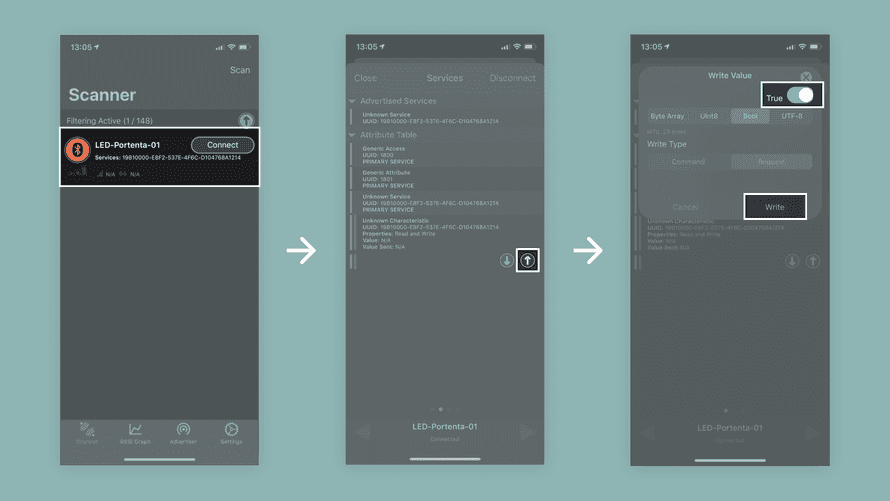
\includegraphics[width=0.7\linewidth]{Images/PortentaH7/Bluetooth-scan.png}
			\caption{Bluetooth-scan}
			\label{Bluetooth-scan} \cite{bluetoothPortentaH7:2024}
		\end{center}
	\end{figure}
	\item \textbf{6. Conclusion:} This example shows how to connect and control the built-in LED using a Bluetooth Low Energy connection. You have learned how a simple Bluetooth Low Energy connection between your Portenta and your cell phone, which has basic communication abilities between the two devices, works. ~\ref{NRF-Connect}	 \cite{bluetoothPortentaH7:2024}
	
\end{itemize}




